\section{Methods}

This section will describe the specific method that we developed to generate lattice-grammars that generate environments.

Before explaining the method we need to clear up some definitions:
By \textit{lattice}, we mean a graph whose nodes are superimposed on a
(potentially infinite) square grid. More precisely, a lattice is a graph whose
nodes are coordinates in 2 dimensional Cartesian space, limited to $\{(x,y) \in
\mathbb{Z} \times \mathbb{Z}\}$, and which may have edges only between nodes
whose euclidean distance is exactly 1.

By \textit{maze} we mean a space of contiguous positions (discrete or not) that 
can be subdivided by walls in any fashion. The environment, in the context of this method, is synonomous with the maze.

The overall method we use for generating mazes can be described as follows:

\begin{enumerate}
	\item We first discover interesting grammars that fit a criteria, using an evolutionary algorithm.
	\item We create lattices from grammars by applying them recursively, each describing the overall layout of a maze
	\item We create mazes from lattices. Each node in the lattice
		corresponding to a fixed-size room in the maze, connected to
		other blocks as described by the lattice.
\end{enumerate}

The three steps each involve multiple variables that can be tweaked in accordance
with with the type of maze one wishes to obtain.


\subsection{Lattice grammars}
A lattice grammar consists of a set of rules, where a rule is defined by a left-
and a right-hand lattice $(r_p, r_r)$. When a rule $(r_p,r_r)$ is applied to a
lattice, $r_p$ is used as a search pattern in the lattice.
If a match is found, the matching part of the lattice is transformed 
into $r_r$. The lattice is transformed by adding edges that are in $r_r$ but
not in $r_p$, and removing edges that are in $r_p$ but not in $r_r$.

An example of a grammar rule is shown in figure \ref{fig:simplerule}, and an
example of applying that rule to a lattice is shown in figure
\ref{fig:simplerule-applied}. In figure \ref{fig:simplerule-applied}, the rule
has been rotated 90-degrees counter-clockwise to find the match, and the lattice
is transformed accordingly to that rotation. Note that this is not the only
match in the lattice. A different, perhaps more obvious, match exists without
rotation.

\begin{figure}[hbp]
	\centering
	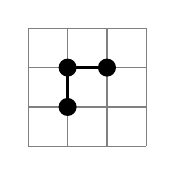
\begin{tikzpicture}
	%grid
	\draw [black!50,step=0.5] (0, 0) grid (1.5, 1.5);

	%nodes
	\foreach \p in {
		(0.5, 0.5),
		(0.5, 1),
		(1.0, 1)
	}\draw [thick, fill=black] \p circle (0.1);

	%paths
	\draw [very thick, color=black] plot coordinates {
		(0.5, 0.5)
		(0.5, 1)
		(1.0, 1)
	};

\end{tikzpicture}
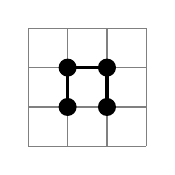
\begin{tikzpicture}
	%grid
	\draw [black!50,step=0.5] (0, 0) grid (1.5, 1.5);

	%nodes
	\foreach \p in {
		(0.5, 0.5),
		(0.5, 1),
		(1.0, 1),
		(1.0, 0.5)
	}\draw [thick, fill=black] \p circle (0.1);

	%paths
	\draw [very thick, color=black] plot coordinates {
		(0.5, 0.5)
		(0.5, 1)
		(1.0, 1)
		(1.0, 0.5)
	};

\end{tikzpicture}

	\caption{The left- and right-hand sides $(r_p,r_r)$ of a lattice-grammar rule that
	adds an edge}
	\label{fig:simplerule}
\end{figure}

\begin{figure}[hbp]
	\centering
	\input{graph-apply-plot.tex}
	\caption{A lattice that is matched by the rule in figure
	\ref{fig:simplerule} (left), and one possible result of applying the
	rule to the lattice (right)}
	\label{fig:simplerule-applied}
\end{figure}

The matching of a rule on a lattice might be implemented without rotation.
Without rotation in the matching process, the choice is deferred to the grammar,
which may or may not include different rotations of a rule. Intuitively,
including rotation in the matching process makes grammars less expressive, but
may help cause self-similarities in the resulting lattice. In practice, the
effect is not entirely obvious, and is tied to the method used to discover
grammars.

Another problem is how a grammar is applied. That is, in
addition to how a single rule is applied, there is the question of how the set
of rules that constitute a grammar is applied. If rules are applied in
succession, the order is significant, as one rule may alter the lattice in a way
that changes how the next rule applies. Of course, this is only true if
application may be done in-place, updating the lattice immediately with each
application. Alternatively, rules could be matched, and then applied together in
a single step. Furthermore, rules may be applied once, or once for each match.
Yet another approach could be to apply each rule repeatedly, continuing to the
next rule only when the first can't be matched to it's own result anymore.

\subsection{Block generation}

The lattice graph describes the overall layout of the maze, but by considering the lattice's nodes as fixed-size rooms, or "block", we can decouple the details of the maze layout from the overall structure. 

Depending on the block-size, this stage of the generation can have a profound impact on the final result. The connectivity of the maze could potentially be altered here, and the depth of cul-de-sacs can be decided, both of which heavily alter the way the level plays.

To ensure that the blocks do not affect the overall level structure too much, the mock algorithm that we use simply removes walls randomly until every exit is connected. This should result in fairly connected room and guarantees that no parts of the environment is cut off unnecessarily.

The blocks are in the algorithm do demonstrate the possibility of a system like what the game Spelunky uses \cite{yu2016spelunky}. A system like this allows the developer to generate the details of the environment independently from the overall structure, for example by authoring rooms manually and then assembling them to a level procedurally. The implementation here is just a mock-up and are not intended to have any effect on the result.


\subsection{Evolutionary algorithm}

We're using a very basic evolutionary algorithm to develop lattice-grammars that will generate environments that fit certain criteria. The overall algorithm looks like this:
\begin{itemize}
\item An initial population is created.
\item Until an termination criteria is met:
\begin{itemize}
    \item Evaluate the population
    \item Select the best from the population to be parents for the next generation
    \item Create randomly mutated offspring from selected individuals
\end{itemize}
\end{itemize}

Each individual in a population is a list of rules that can be applied. They
start out as empty rules that replaces nothing with nothing. The mutations that
can be performed will then add or remove edges from the rules, or add another
empty rule to the list. This is the genotype that will generate a lattice graph,
the genotype.

To evaluate the population we use a mix of different metrics in a fitness
function. Novelty search may also be a viable option, but was outside the
scope of the project. The different metrics are weighted depending on which
features of the graph should have the most influence.

For the selection process, the top 50\% ranking of the population is picked.
This is one of the most basic elitist selection methods, but it's enough for us
to achieve decent results, by simply discarding the individuals that did not
mutate in a beneficial fashion.

Offspring generation is a-sexual. The 50\% highest ranking individuals are taken
together in pairs, and in lieu of crossover, we simply copy one parent at
random.
An actual crossover algorithm might improve the results, but because was not
necessary.
If we were to extend the algorithm with actual breeding, we would take
inspiration from the NEAT algorithm\cite{stanley:ec02}, to get proper crossover
when combining graphs.

Finally, the offspring are mutated at random, and together with the selected
individuals they form the next generation.

The evolution algorithm terminates after a certain number of generations, after which the best five mazes will be shown.

\subsection{Experiments}
In order to meet the criteria described in section \ref{sec:mechanics}, we run
several evolutionary experiments, with different fitness criteria.
A few small variations of the fitness functions were used, but we outline the
"final" two in the sections below, and in the result section, we'll point to
which results came specifically from the functions shown here.

\subsubsection{Cops and Robbers}
For games in the Cops and Robbers category, we try to evolve grammars that have
few but some pitfalls, few cul-de-sacs and a small average travel distance
between nodes. This should favour high-connectivity mazes with a few dead-ends,
providing "don't think just run" levels, sprinkled with a few traps created by
cul-de-sacs and pitfalls.

The final fitness function used was a sum of the following terms:
$$-\left|(30.0-size)^{1.3}\right|$$

$$- 30.0 * \frac{pitfalls}{size}$$

$$-\frac{medianDistance}{1 + \sqrt{area}}$$

$$-\left| 50 * \left(0.05 - \frac{culdesacs}{size}\right)\right|$$
$$-\left| 3 - \max culdesaclength \right|$$

For a lattice, where $size$ is the number of nodes, $pitfalls$ is the number of
pitfall nodes (as defined previously), $medianDistance$ is the median of all
node distances, and $\max culdesaclength$ is the length of the longest path
on a cul de sac.

Where necessary, $0$ is substituted for terms resulting in division with $0$.

\subsubsection{Dungeon Crawlers}
For games in the Dungeon Crawler category, we try to evolve grammars that are
rich in cul-de-sacs and large trees, with a comparatively low degree. This
should favour mazes that consist of disjunct parts, and with "narrow" paths and
choke-points.

The final fitness function used was a sum of the following terms:
$$-\left|(30.0-size)^{1.3}\right|$$
$$trees$$
$$treeLength^\prime$$
$$log_{1.02} \left(\frac{treeLength^\prime}{culdesaclength^\prime} \right)$$
$$- 12^{\left| 2.5 - avgDegree \right|}$$

Where $treeLength^\prime$ is the median size of trees, $culdesaclength^\prime$
is the median length of cul de sacs, and $avgDegree$ is the average number of
connected neighbours a node has.

A tree is defined as a sub graph with no cycles, where all nodes have at most 2
connected neighbours, with the exception for one node, considered to be the root of three.

$trees$ is the number of such trees.

Where necessary, $0$ is substituted for terms resulting in division with $0$.
